\documentclass
[
	8pt,		% font size
	ngerman,	% hyphenation and more
	a4paper,	% paper size
	landscape,	% orientation
	final		% document status (final/draft)
]{extarticle}

% \newenvironment{graphics}
%   {\par\medskip\noindent\minipage{\linewidth}}
%   {\endminipage\par\medskip}

% adjust language %
\usepackage[ngerman]{babel}
% integration of speacial characters %
\usepackage[utf8]{inputenc}
\usepackage[T1]{fontenc}
\usepackage{textcomp}
% adjust page layout %
\usepackage{titlesec}
\usepackage{fancyhdr}
% --------------------------- %
\usepackage{multicol}
\usepackage{multirow}
% --------------------------- %
\usepackage{setspace}
\usepackage{geometry}
\usepackage{adjustbox}
% adjust colors %
\usepackage{color}
% integration of mathematical symbols %
\usepackage{amsmath}
\usepackage{amssymb}
\usepackage{amsthm}
\usepackage{mathtools}
% integration of source code %
\usepackage{listings}
% adjust enumerations %
\usepackage{enumitem}
% adjust tables %
\usepackage{tabularx}
% integration of graphics %
\usepackage{graphicx}
% create graphics %
\usepackage{tikz}
\usetikzlibrary{automata, positioning, arrows}
% integration of seperate files %
\usepackage{standalone}

% ========== INFORMATION ========== %
\def\name{Louis Seubert}
\def\prefix{Zusammenfassung}
\def\lecture{Interaktivesysteme}
\def\maxpages{6}

% ============== ADJUSTMENTS ============== %
% adjust graphics path %
\graphicspath
{
	{figures/}
}
% adjust page layout %
\geometry
{
	left=0.55cm,
	right=0.55cm,
	top=1.10cm,
	bottom=0.55cm,
	headsep=2mm
}
% adjust source code view %
\lstset
{
	basicstyle=\ttfamily\footnotesize,
	columns=fullflexible,
	numbers=left,						% where to put the line-numbers
	numberstyle=\tiny,  				% the style that is used for the line-numbers
	stepnumber=1,
	numbersep=5pt,						% how far the line-numbers are from the code
	showspaces=false,					% show spaces adding particular underscores
	showstringspaces=false,				% underline spaces within strings
	showtabs=false,						% show tabs within strings adding particular underscores
	frame=none,							% adds a frame around the code
	tabsize=2,							% sets default tabsize to 2 spaces
	captionpos=b,						% sets the caption-position to bottom
	breaklines=true,					% sets automatic line breaking
	breakatwhitespace=false,			% sets if automatic breaks should only happen at whitespace
	xleftmargin=10pt					% left margin to prevent number clipping
}

% make header and footer %
\pagestyle{fancy}
\fancyhead{} % clear header
\fancyhead[L]{\prefix\;\lecture}
\fancyhead[R]{\thepage\;--\;\maxpages}
\fancyhead[C]{\name}
\fancyfoot{} % clear footer

% configure document %
\setitemize{leftmargin=15pt}
\setenumerate{leftmargin=15pt}
\setlist{itemsep=1pt,parsep=1pt,noitemsep}

\setlength{\parindent}{0pt}
\setlength{\parskip}{0pt}
\setlength{\topskip}{10pt}
% set column seperator %
\setlength{\columnseprule}{0.5pt}

% change style %
\titleformat*{\section}{\large\bfseries}
\titlespacing*{\section}{0pt}{4pt}{0pt}

\titleformat*{\subsection}{\normalsize\bfseries}
\titlespacing*{\subsection}{0pt}{4pt}{0pt}

\titleformat*{\subsubsection}{\normalsize\bfseries}
\titlespacing*{\subsubsection}{0pt}{4pt}{0pt}

\titleformat*{\paragraph}{\normalsize\bfseries}
\titlespacing{\paragraph}{0pt}{.5em}{.5em}

\titleformat*{\subparagraph}{\small\bfseries}
\titlespacing*{\subparagraph}{0pt}{.5em}{.5em}

% define some macros %
\newcommand{\example}{\textit{\underline{Beispiel:} }}

% define some enviroments %
\newenvironment{definitions}{
	\par\vspace{\abovedisplayshortskip}\noindent
	\tabularx{\columnwidth}{>{$}l<{$} @{${}={}$} >{\raggedright\arraybackslash}X}
}{
	\endtabularx\par\vspace{\belowdisplayshortskip}
}

\hyphenation{
	Zei-ge-ge-rä-tes
	zwei-di-men-si-o-nal
	mehr-di-men-si-o-nal
	Ge-nau-ig-keit
	mehr-deu-ti-ge
	ba-sie-ren
	Er-schei-nung
	bei-tra-gen
	meh-re-rer
	in-vol-vier-ten
	Än-der-ungs-auf-trä-ge
	Im-ple-men-tie-rung
	re-du-zier-ten
	Ent-kopp-lung
	In-ter-ak-ti-ons-mo-dell
	Ein-ga-ben
	Ein-ga-be-fol-gen
	Funk-ti-o-nen
	Be-nut-zer-schnitt-stel-le
	Be-zie-hun-gen
	ato-ma-rer
}

\begin{document}
\begin{multicols*}{4}
	\section{Einführung}
	\subsection{Unterscheidung Anwender \(\leftrightarrow\) Benutzer}
	\begin{description}
		\item[Anwender] sind Entitäten, welche direkt oder auch indirekt ein
		      Hilfsmittel zur Erzielung eines Vorteils verwendeen
		\item[Benutzer] sind natürliche Personen, die direkt mit einem
		      Hilfsmittel arbeiten, um einen Vorteil zu erzielen
	\end{description}
	\example Ein Direktor (Anwender) lässt sich von seinem Chauffeur (Benutzer)
	mit einem Auto (Hilfsmittel) zu seinem nächsten Termin bringen
	\subsection{Definition Interaktives System}
	Ein \textbf{interaktives System} gibt dem Benutzer die Möglichkeit, mittels
	einer Benutzerschnittstelle die laufende Bearbeitung einer Aufgabe durch ein
	technisches System zu beeinflussen.
	\subsection{Formen von Interaktion}
	\begin{itemize}
		\item \textbf{Anweisung}
		      \begin{itemize}
			      \item Eingabe von Kommandos
		      \end{itemize}
		\item \textbf{Dialog}
		      \begin{itemize}
			      \item Ablauf von Eingabe und Ausgabe
		      \end{itemize}
		\item \textbf{Manipulation (von Kommandos, Inhalten)}
		      \begin{itemize}
			      \item Auswählen („Choice“)
			      \item Ansteuern („Target Acquisition“)
			      \item Verändern
		      \end{itemize}
		\item \textbf{Erkunden (einer Menge von Kommandos, Inhalten)}
		      \begin{itemize}
			      \item Suchanfragen
			      \item Browsing
		      \end{itemize}
	\end{itemize}
	\subsection{Arten von Benutzerschnittstellen}
	\begin{itemize}
		\item \textbf{T}ext \textbf{U}ser \textbf{I}nterface
		\item \textbf{T}angible \textbf{U}ser \textbf{I}nterface
		\item \textbf{G}raphical \textbf{U}ser \textbf{I}nterface
		\item \textbf{V}oice \textbf{U}ser \textbf{I}nterface
		\item \textbf{H}aptic \textbf{U}ser \textbf{I}nterface
		\item \textbf{N}atural \textbf{U}ser \textbf{I}nterface\par
		      (möglichst wenig zu erlernende Eingabegeräte)
		\item \textbf{I}ntuitive \textbf{U}ser \textbf{I}nterface\par
		      (möglichst leicht erlernbare Eingabegeräte)
		\item \textbf{B}rain \textbf{C}omputer \textbf{I}nterface
		\item \textbf{C}ommand \textbf{L}ine \textbf{I}nterpreter
	\end{itemize}
	\subsection{Fallstudien}
	\subsubsection*{Sketchpad}
	Programm entwickelt von Ivan Sutherland im Rahmen einer Doktorarbeit. \\
	Mittels Lichtgriffel: Zeichnen und Deformieren geometrischer Objekte;
	Vektorgraphiken; Erste objektorientierte Ansätze zur Bedienung
	\subsubsection*{Xerox Alto}
	Kommandozeileninterpreter Alto Executive: Graphische Oberfläche;
	Mehrere Applikationen; Mehrere Fenster
	\subsubsection*{Apple Macintosh}
	Features u.a. Desktop-Metapher, Drop-Down-Menüs, Ordner, Mülleimer sowie
	überlappende Fenster
	\subsubsection*{Windows 1.0}
	Zeigegerät, Menüs, Statuszeile, Symbole, Zwischenablage, Taskleiste.
	Wegen Vektorgrafik-Fähigkeit bereits als GUI (und nicht als TUI)
	klassifiziert.
	\section{Zeigegeräte}
	\subsection{Einteilung von Interaktionstechnologien}
	Nach \emph{Krauß}
	\begin{itemize}[nolistsep]
		\item Koordinatengebend
		      \begin{itemize}[nolistsep]
			      \item Dimensionalität
			            \begin{itemize}[nolistsep]
				            \item[\(\rightarrow\)] eindimensional,
				                  zweidimensional, mehrdimensional
			            \end{itemize}
			      \item Verhältnis Lage zu Wirkort
			            \begin{itemize}[nolistsep]
				            \item[\(\rightarrow\)] Indirekt wirkende vs. direkt
				                  wirkende
			            \end{itemize}
		      \end{itemize}
		\item Nicht koordinatengebend
		      \begin{itemize}[nolistsep]
			      \item Tasten
			      \item Sprache
			      \item Gesten
		      \end{itemize}
	\end{itemize}
	\subsection{Koordinatengebende}
	\subsubsection{Direkte Zeigegeräte}
	\begin{itemize}
		\item Es wird unmittelbar auf die Ausgabe gezeigt
		\item Merkmale
		      \begin{itemize}[nolistsep]
			      \item Lernaufwand Bedienung Zeigegeräts minimal
			      \item Verdeckung der Ausgabe durch Zeigegerät
			      \item Ermüdungserscheinungen
		      \end{itemize}
		\item \example Touchscreen
	\end{itemize}
	\subsubsection{Indirekte Zeigegeräte}
	\begin{itemize}
		\item Nicht im direkten Kontakt mit der Ausgabe
		\item Bewegung an anderer Stelle und Transformation der Koordinaten an
		      den Bildschirm
		\item Merkmale
		      \begin{itemize}[nolistsep]
			      \item Lernaufwand Bedienung des Zeigegeräts \\
			            z.B. Hand-Augen-Koordination bei Computermaus
			      \item Kopplung zwischen Zeigegerät und Ausgabe als
			            modulierbarer Parameter
		      \end{itemize}
		\item \example Computermaus
	\end{itemize}
	\subsubsection{Positionierung}
	\paragraph{Absolute Positionierung} Eindeutige Zuordnung der Position des
	Zeigegerätes zur Position auf dem Bildschirm. Der Bezug zum Ursprung kann
	gegeben sein.
	\paragraph{Relative Positionierung} Es wird von aktuell gespeicherter
	Position ausgegangen und die Veränderung der Koordinaten umgesetzt.
	\paragraph{Control-Display-Gain} \textbf{<<MacKenzie>>} Der durch die
	Bewegung eines indirekten Zeigegerätes ("Control") resultierende Effekt
	(„Gain“) am Bildschirm. \\
	Nach MacKenzie balanciert eine günstige Einstellung des Gain Schnelligkeit
	und Präzision der Positionierung.
	\begin{center}
		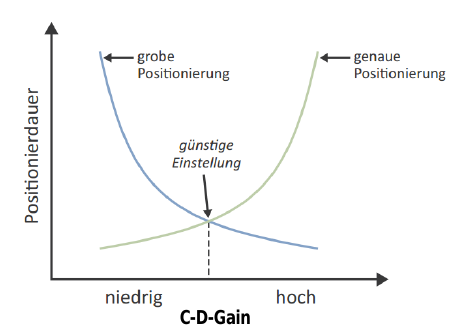
\includegraphics[width=0.7\linewidth]{./Documents/Graphics/ControlDisplayGain.png}
	\end{center}
	\begin{itemize}
		\item \textit{Gain niedrig:} Große Bewegung Controller bewirkt
		      durchschnittlichen Effekt; Vorteilhaft für Feinpositionierung
		\item \textit{Gain hoch:} Kleine Bewegung Controller bewirkt
		      durchschnittlichen Effekt; Vorteilhaft für Grobpositionierung
	\end{itemize}
	\subsubsection{Physikalische Charakterisierung}
	\paragraph{Abtastrate}
	\begin{itemize}
		\item Erfassung der Position und Tasten des Zeigegerätes zu diskreten
		      Zeitabständen
		\item Definiert die zur Positionsbestimmung verfügbare Zeit
	\end{itemize}
	\begin{center}
		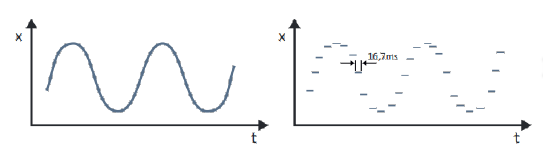
\includegraphics[width=\linewidth]{./Documents/Graphics/SamplingRate.png}
	\end{center}
	\paragraph{Verzögerung}
	\begin{itemize}
		\item Zeitabstand zwischen Abtastung und Änderung am Bildschirm
		\item Verzögerung sollte geringer als die Hälfte der Abtastrate sein
		\item Schon geringe Verzögerungen bringen höhere Fehlerrate bei
		      Selektionen mit sich
	\end{itemize}
	\paragraph{Genauigkeit}
	\begin{itemize}
		\item Genauigkeit: Abweichung der durch einen Sensor gemessenen Position
		      von der tatsächlichen Position
		\item Gemeinsame Optimierung von Genauigkeit und Abtastrate nicht
		      möglich
		      \begin{itemize}[nolistsep]
			      \item Obergrenze bildet die räumliche Auflösung des Sensors
			      \item Hohe Abtastrate geht zu Lasten der Genauigkeit
		      \end{itemize}
	\end{itemize}
	\paragraph{Abhängigkeit von der individuellen Anwendung}
	\begin{itemize}
		\item Bei Interaktion in komplexen virtuellen Welten in modernen
		      Computerspielen oder 3D-Modellierungstools können hohe
		      Anforderungen an Zeigegeräte gestellt werden
	\end{itemize}
	\subsubsection{Zeige Aufgaben}
	\begin{center}
		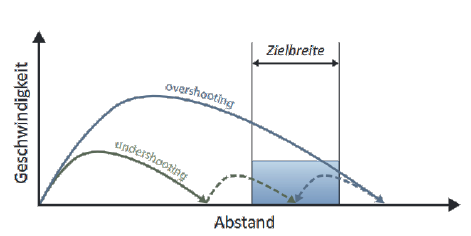
\includegraphics[width=0.7\linewidth]{./Documents/Graphics/TargetSelectionTask.png}
	\end{center}
	Das Experiment nach Fitts: Wie lange benötigt ein Mensch \(MT\), um mit einm
	Stift ausgehend von einem Startpunkt ein Ziel zu erreichen? Das Experiment
	steht dabei in der Abhängigkeit von der Distanz \(D\) des Ziels und der
	Breite \(W\).
	\paragraph{Fitts}
	\[MT = a + b \cdot ID\]
	\[ID = \log_{2}\left(\frac{2D}{W}\right)\]
	\paragraph{MacKenzie}\mbox{}\\
	Verbesserung der Formel von Fitts
	\[ID = \log_{2}\left(\frac{D}{W} + 1\right)\]
	\paragraph{Accot \& Zhai}\mbox{}\\
	Berücksichtigt auch Höhe und y-Koordinate des Ziels
	\[MT = a + b \cdot \log_{2}\left(\sqrt{\left(\frac{D}{W}\right)^{2}+\eta\left(\frac{D}{H}\right)^{2}} + 1\right)\]
	\subsubsection{Ergebnisse des Praktikumsversuchs}
	MacKenzie > Accot/Zhai > Fitts
	\begin{itemize}
		\item In Fitts' Experiment wird ein direktes Zeigegerät benutzt
		\item \emph{Precuing} macht eine Zeigeaufgabe immer einfacher
		\item \emph{Reset} macht eine Zeigeaufgabe zunächst schwerer, jedoch
		      kann es schnell erlernt werd
	\end{itemize}
	\subsubsection{Unterstützung von Zeigeaufgaben}
	\paragraph{Anpassung Bedienelemente} Eine Anpassung der Größe, Anordnung,
	Form. \\ Verkleinern ist nach Fitts schwieriger und die Unterscheidbarkeit
	nimmt ab.
	\paragraph{Temporäre Modifikation des Interface} Eine Anpassung des User
	Interface. \\ Nach Parker kann man das Ziel oder den Cursor vergrößern,
	sowie den Cursor zum Ziel bewegen oder auch das Ziel zum Cursor bewegen. \\
	\underline{Nachteile:} Eine Veränderung des User Interface kann den Benutzer
	irritiren; Aussagen über eine Selektionsinteraktion sind schwer
	\paragraph{Mehrere Mauszeiger} \underline{Nachteile:} Potentiell mehrdeutige
	Zielauswahl
	\subsubsection{Direct Manipulation}
	Direkt manipulative Interfaces zeichnen sich aus nach \emph{Hutchins et al.}
	durch:
	\begin{itemize}
		\item Geringe Distanz
		      \begin{itemize}[nolistsep]
			      \item von Benutzerzielen
			      \item zu deren Erreichung nötigen Interaktionen
		      \end{itemize}
		\item Hohes Engagement
		      \begin{itemize}[nolistsep]
			      \item direkte Auseinandersetzung des Benutzers
			      \item mit dem Objekt von Interesse
		      \end{itemize}
		\item \example
		      \begin{itemize}[nolistsep]
			      \item Skript schreiben:\\ Distanz hoch, Engagement niedrig
			      \item Drag \& Drop:\\ Distanz niedrig, Engagement hoch
		      \end{itemize}
	\end{itemize}
	\paragraph{Prinzipien nach Shneiderman}
	\begin{itemize}
		\item Kontinuierliche Repräsentation des Objekts von Interesse
		\item Eingabe auf Basis einfacher physikalische Aktionen
		      (z.B. Bewegung der Maus) anstelle sprachbasierter Kommandos
		\item Schnelle, schrittweise, umkehrbare Operationen, deren Auswirkung
		      auf das Objekt von Interesse unmittelbar erkennbar wird
		\item Schrittweises Erlernen der Interaktion ausgehend von minimalem
		      Vorwissen
	\end{itemize}
	\paragraph{Vorteile nach Shneiderman}
	\begin{itemize}
		\item Anfänger können die grundlegende Funktionen schnell erlernen,
		      beispielsweise nach Vorführung durch einen erfahreneren Benutzer
		\item Interaktionskonzepte werden nach längerer Nichtanwendung leicht
		      erinnert
		\item Benutzer können unmittelbar erkennen, ob sie sich durch Aktionen
		      ihren Zielen annähern – und gegebenenfalls ihre Aktionen anders
		      ausrichten
		\item Benutzer sind weniger zögerlich im Umgang mit dem System, da
		      Aktionen leicht verständlich und umkehrbar sind
		\item Benutzer erleben Kontrolle über das System und können dessen
		      Reaktionen direkt beobachten
	\end{itemize}
	\subsection{Nicht koordinatengebend}
	\subsubsection{Sprachbasierte Interaktionsformen}
	Nach \emph{Preim \& Dachselt}
	\begin{itemize}
		\item Kommandosprachen
		\item Textuelle Suche
		\item Natürlich-sprachliche Systeme
	\end{itemize}
	\paragraph{Phoneme \& Prosodie}\mbox{}\\
	\underline{Phonem:} “Phoneme sind die kleinsten bedeutungsunterscheidenden
	Einheiten einer Sprache." \\ Der Austausch eines Phonems ändert die Bedeutung
	eines Wortes.
	\underline{Prosodie:} "Prosodie ist die Gesamtheit derjenigen lautlichen
	Eigenschaften der Sprache, die nicht [...] ans Phonem als minimales Segment,
	sondern an umfassendere lautliche Einheiten gebunden sind" \\ Dient u.a. der
	Kennzeichnung des Satztyps (z.B. Frage, Aussage), Gewichtung oder Gliederung.
	\paragraph{Spracherkennung} \underline{Audiosignal \(\rightarrow\) Text}
	\begin{itemize}
		\item Vorverarbeitung (Filterung um Störgeräusche zu extrahieren,
		      Frequenzspektrum berechnen, Sprachrelevante Merkmale extrahieren)
		\item Extraktion von Phonemen
		\item Abbildung von Phonemfolgen auf Wörter
	\end{itemize}
	\paragraph{Semantische Analyse} Bedeutung der Aussage auf struktureller
	Ebene (Agenten, Handlungen, Intentionen, Objekte), Ergebnis unter Umständen
	nicht eindeutig
	\paragraph{Pragmatische Analyse} Bedeutung der Aussage im Kontext, z.B. Ort,
	Zeit, Fähigkeiten, Intention; Hinzuziehen weiterer Sprachmerkmale (Prosodie);
	auch hier Ergebnis unter Umständen nicht eindeutig
	\paragraph{Sprachsynthese} \underline{Text \(\rightarrow\) Audiosignal}
	\begin{itemize}
		\item NLP (Natural Language Processing) transkribiert Text anhand eines
		      Phonem-Alphabets und einer Prosodiebeschreibung
		\item DSP (Digital Speech Processing) synthetisiert aus der NLP-Ausgabe
		      das Audio-Signal gesprochener Sprache
	\end{itemize}
	Ansätze für die Umsetztung:
	\begin{itemize}
		\item Modellbasierte Synthese: erzeugt ein Audio-Signal auf Basis eines
		      Modells
		\item Konkatenative Synthese: verknüpft Ausschnitte aus Aufzeichnungen
		      gesprochener Sprache um zu einem neuen Audiosignal
	\end{itemize}
	\subsubsection{Tastatur}
	Die Effizienz hängt ab von ...
	\begin{itemize}
		\item[...] Größe, Form und Position der Tasten
		\item[...] Art der Eingabe (Symbolhäufigkeiten und Symbolfolgen), im
		      Fall natürlicher Sprache also von der Sprache, in der der Text
		      verfasst wurde
		\item[...] Technologischen Randbedingungen
	\end{itemize}
	Die \textbf{QWERTY} Tastenbelegung orientierte sich danach das sich in der
	Englischen Sprache die Typenhebel einer Schreibmaschiene nicht kollidierten.
	\paragraph{Virtuelle Tastaturen}
	\begin{itemize}
		\item Platzersparnis: z.B. Temporäres Einblenden bei Touch-Interaktion
		      genau dann, wenn alphanumerische Eingaben benötigt werden
		\item Konfigurierbarkeit: z.B. Tastaturen, deren Layout sich anpasst
	\end{itemize}
	\underline{Probleme:} Fat Finger Problem, Fehlender Druckpunkt
	(Tasten können versehentlich ausgelöst werden)
	\section{Graphische Dialogsysteme}
	\subsection{WIMP-Prinzipien}
	\textbf{WIMP}: \underline{\textbf{W}indows \textbf{I}cons \textbf{M}enus \textbf{P}ointer}
	\begin{description}
		\item[Metaphors] Interaktionsmechanismen werden auf bekannte
		      Arbeitsabläufe abgebildet
		\item[Direct Manipulation] Der Benutzer soll direkt mit Objekten der
		      Benutzerschnittstelle interagieren können
		\item[See and Point] Die Interaktion mit der Maschine soll auf den
		      gerade sichtbaren Objekten basieren
		\item[Consistency] Objekte mit ähnlicher Funktion sollen ähnlich
		      aussehen und sich ähnlich verhalten
		\item [User Control] Nur der Benutzer soll Aktionen der Maschine
		      initiieren und deren Ablauf kontrollieren
		\item [Feedback and Dialog] Alle ausgeführten Aktionen des Benutzers
		      und deren Effekte sollen ohne Verzögerung erkennbar sein
		\item [Forgiveness] Aktionen des Benutzers sollen rückgängig gemacht
		      werden können, bei kritischen Aktionen soll gewarnt werden
		\item [Aesthetic Integrity] Das Erscheinungsbild der Benutzeroberfläche
		      soll einfach, aufgeräumt und konsistent sein
		\item [Modelessness] Der Benutzer soll alle möglichen Aktionen zu jedem
		      Zeitpunkt ausführen können. (Aufwendig zu implementiren)
		\item [WYSIWYG] Dokumente sollen bei der Erstellung so angezeigt werden,
		      wie sie als Ausdruck ausgegeben werden. (\textbf{Nur Drucker!})
	\end{description}
	\subsection{Fenster}
	\begin{itemize}
		\item Rechteckige Bereiche, die Interaktionen von Benutzern verarbeiten
		      können
		\item Präsentation und Verhalten angelehnt an Metapher „Papier“
		      \begin{itemize}[nolistsep]
			      \item stapelbar, verschiebbar
			      \item Passend zur Metapher „Schreibtisch“
			      \item Historisch in Büroarbeiten begründet
		      \end{itemize}
		\item Begriff verdeutlicht die Funktion einer Sicht („View“) auf Objekte
		      einer Anwendung
	\end{itemize}
	\subsubsection{Varianten}
	\begin{description}
		\item[Applikationsfenster] Beinhaltet (logisch) alle Bedienelemente
		      einer Anwendung
		\item[Dialogfenster] Informieren oder Aufforderung zur Eingabe
		\item[Elementares Fenster (Widget)] Die jenigen Bedienelemente, die eine
		      Einheit aus Erscheinung und zugehörigem Verhalten bilden
	\end{description}
	\subsubsection{Verwaltung von Fenstern}
	\begin{itemize}
		\item Window Manager sind entweder im Fenstersystem integriert, oder
		      können auch austauschbar sein
		\item Realisieren das Verschieben, Skalieren, Öffnen und Schließen der
		      Fenster
		\item Steuern das Aussehen der Fenster, d.h. die Gestaltung der
		      Titelzeile und der Scrollbars
		\item Realisieren Fensterplatzierungsstrategien
		\item Unterstützen Navigation in Fenstern
	\end{itemize}
	\subsubsection{Koordinatensysteme}
	Das Koordinatensystem eines Fenstersystems bestimmt Positionierung und Größe
	präsentierter Information
	\begin{description}
		\item[Geräteabhängige Koordinaten] Die Koordinaten auf einem gegebenen
		      Ausgabegerät
		\item[Geräteunabhängige Koordinaten] Die Entkopplung der Präsentation
		      von geräteabhängigen Parametern (insbesondere: Auflösung) der
		      Ausgabegeräte \\
		      \example Eine 1 cm Linie soll auf einem Bildschirm mit 150 dpi
		      genauso lang ausgegeben werden wie auf einem Drucker mit 2400 dpi
		\item[Weltkoordinaten] Entkopplung der Präsentation von der
		      Repräsentation der zugrundeliegenden Daten \\
		      \example Sowohl Nanometer für Moleküle wie auch astronomische
		      Koordinaten sollen vom Modell abgebildet werden können
	\end{description}
	\subsection{Piktogramme}
	\begin{itemize}
		\item Symbole, die Komponenten eines Fenstersystems graphisch
		      repräsentieren
		\item Orientierung an bildhaften Darstellungen in anderen Bereichen der
		      natürlichen Umgebung
		      \begin{itemize}[nolistsep]
			      \item Ziel: Ausnutzen der ausgeprägten Stärke des Menschen,
			            erlernte Muster (wieder) zu erkennen
		      \end{itemize}
		\item Unabhängigkeit von einer bestimmten Sprache
		      \begin{itemize}[nolistsep]
			      \item Können damit zur Internationalisierung beitragen
		      \end{itemize}
	\end{itemize}
	\subsubsection{Varianten}
	\begin{description}
		\item[Repräsentative Piktogramme] Stellen einen abstrakten Sachverhalt
		      bzw. ein Konzept dar \\
		      \example Symbole für Mülleimer, Disketten, Drucker
		\item[Abstrakte Piktogramme] Stellen einen abstrakten Sachverhalt bzw.
		      ein Konzept dar und müssen somit erst erlernt werden \\
		      \example Symbole für Pfeile, Wiederholung, Rückgängig
		\item[ Hybride Formen] Stellen eine Mischform da
	\end{description}
	\subsubsection{Richtlinien}
	\begin{itemize}
		\item Einfachheit und Klarheit
		\item Verständlichkeit
		\item Einprägsamkeit
		\item Platzsparende Gestaltung
		\item Klarer Kontrast zu Hintergrund
		\item Hohe Unterscheidbarkeit vs. Konsistenz
		\item Selektierter Zustand sollte klar ersichtlich sein
	\end{itemize}
	\subsection{Menüs}
	\begin{itemize}
		\item Basieren auf Hierarchien und Taxonomien
		\item Dienen dem Auslösen atomarer Aktionen
		\item Komplexere Interaktionen wie die Eingabe mehrerer Werte etc.
		      durch die Verbindung mit Dialogen
	\end{itemize}
	\paragraph{Motivation}
	\begin{itemize}
		\item Es soll unter einer endlichen Menge von Aktionen gewählt werden
		\item Man soll die Menge der Aktionen nicht erlernen müssen
		\item Man soll im Vermeiden syntaktischer Fehler unterstützt werden
	\end{itemize}
	\subsubsection{Hick \& Hyman}
	Versuchsaufbau ,,choice-reaction time''
	\begin{itemize}
		\item 2-10 Lampen angeordnet in einem irregulären Kreis
		\item Jeder Lampe ist eine Taste zugeordnet
		\item Alle 5 Sekunden leuchtet zufällig eine Lampe auf
		\item Testperson soll zugeordnete Taste drücken
		\item Vorfeld: Testpersonen erlernen Zuordnung
	\end{itemize}
	\paragraph{Hick-Hyman Gesetz}
	\begin{itemize}
		\item Informationsgehalt der Aufgabe (,,choice'')\\
		      \(H = \log_{2}(n)\)
		\item Reaktionszeit (,,reaction time'')\\
		      \(RT = a + b \cdot \log_{2}(n)\)
		\item Reaktionszeit in hierarchischen Menüs folgt dem Hick-Hyman-Gesetz
		      laut Landauer \& Nachbar, 1985
		\item Reaktionszeit bei häufig verwendeten Aktionen folgt dem
		      Hick-Hyman-Gesetz ist aber linear bei selten verwendeten Aktionen
		      laut Sears \& Shneiderman, 1994
		\item Bei Anfängern ist die \(RT\) in einem Menü linear, bei Experten
		      folgt sie dem Hick-Hyman-Gesetz (laut Cockburn \& Gutwin, 2008) \\
		      \textbf{Beachte:} Bei plötzlichen Menü-Änderungen sind auch
		      Experten wieder Anfänger und müssen das Menü neu erlernen!
	\end{itemize}
	\section{Post-WIMP}
	WIMP nimmt eine Anwendungssituation an:
	\begin{itemize}
		\item Benutzer kennt Grundkonzepte von Computern
		\item Benutzer ist konzentriert auf den Computer
		\item Bearbeitung alleine und vom Nutzer getrieben
		\item Hardware = \\ Desktop-PC, Maus, Tastatur, Bildschirm
		\item Büroumgebung \\ (d.h. gute Beleuchtung, wenig Störeinflüsse)
	\end{itemize}
	Diese Voraussetzungen sind in heutigen Anwendungssituationen teilweise nicht
	mehr gegeben daher wandelte sich das WIMP Konzept zu dem heutigem Post-WIMP
	Konzept.
	\subsection{WIMP vs. Post-WIMP}
	\begin{tabularx}{\linewidth}{|l|X|} \hline
		WIMP                & Post-WIMP                                                                                  \\\hline
		Metaphors           & Interaktion in der realen Welt                                                             \\\hline
		Direct Manipulation & Delegierung von Aufgaben an das System                                                     \\\hline
		See and Point       & Describe and input Command                                                                 \\\hline
		Consistency         & Diversity; angepasst an den Einsatztort (kann nicht immer angewendet werden)               \\\hline
		WYSIWYG             & Erkennung des Wunsches des Benutzers und der Darstellung einer gleichwertigen Ausgabe      \\\hline
		User Control        & teilweise gegeben oder Shared Control                                                      \\\hline
		Feedback and Dialog & nicht zum Zeitpunkt der Interaktion                                                        \\\hline
		Forgiveness         & User Model; System weiß, was der Nutzer als Ergebnis haben möchte                          \\\hline
		Aesthetic Integrity & oft verletzen von See and Point durch Ausblenden von Inhalten                              \\\hline
		Modelessness        & User Model vorhanden, um Verhalten vorherzusagen; mehrere Funktionen für z.B. einen Button \\\hline
	\end{tabularx}
	\subsection{Touchscreens}
	Technische Varianten: Kapazitiv, resistiv; Singletouch, Multitouch;
	Druckstärke
	\subsubsection{Kapazitive Touchscreens}
	Funktioniert mit einem elektrischen Feld, in fast allen Smartphones \\
	\textit{Vorteil:} lässt sich mit starkem Glas gut vor äußeren Einwirkungen
	schützen
	\subsubsection{Resistive Touchscreens}
	Funktioniert mit zwei Schichten welche aneinander gedrückt werden \\
	\textit{Vorteil:}
	\begin{itemize}
		\item Bedienung mit jedem Eingabestift möglich
		\item Mit Handschuhen und Prothesen bedienbar
		\item Genauer als kapazitive Touchscreens
		\item Geringe Fertigungskosten
	\end{itemize}
	\textit{Nachteile:}
	\begin{itemize}
		\item Nur eingeschränktes Multitouch (Two-touch)
		\item Ist schlecht lesbar bei Sonneneinstrahlung durch Zusatzschicht
		\item Die Gestenbedienung, aufgrund des notwendigen Drucks, ist erschwert.
		\item Verschleiß durch die mechanische Belastung beim Betätigen
		\item Unerwünschtes Auslösen beim Transport durch Kontakt mit anderen
		      Gegenständen möglich
	\end{itemize}
	\section{Entwicklung interaktiver Systeme}
	\subsection{DIN EN ISO 9241-110}
	\begin{tabularx}{\linewidth}{|l|X|} \hline
		\textbf{DIN EN ISO}          & \textbf{WIMP}                              \\\hline
		Aufgabenangemessenheit       & Aesthetic Integrity, See and Point         \\\hline
		Selbstbeschreibungsfähigkeit & Direct Manipulation, Metaphors             \\\hline
		Lernförderlichkeit           & Metaphors, Feedback \& Dialog, Forgiveness \\\hline
		Steuerbarkeit                & User Control                               \\\hline
		Erwartungskonformität        & Consistency, WYSIWYG                       \\\hline
		Individualisierbarkeit       & Modelessness                               \\\hline
		Fehlertoleranz               & Forgiveness                                \\\hline
	\end{tabularx}
	\subsection{Prinzipien der Entwicklung}
	\begin{itemize}
		\item Konzentration auf Benutzer
		      \begin{itemize}[nolistsep]
			      \item Benutzeranalyse
			      \item Umfeldanalyse
			      \item Tätigkeitsanalyse
		      \end{itemize}
		\item Frühes und kontinuierliches Testen
		      \begin{itemize}[nolistsep]
			      \item Erlebbarkeit der Benutzerschnittstelle in Entwurfsphase
			            fördern
			      \item Integriertes Design
			            \begin{itemize}[nolistsep]
				            \item Erheben von Feedback zum Zusammenspiel von
				                  Interaktionselementen bei der Durchführung
				                  typischer Aufgaben der Benutzer
				            \item Solche Test erfordern die volle Verfügbarkeit
				                  aller involvierten Interaktionselemente die
				                  bei herkömmlicher Implementierung erst spät im
				                  Entwicklungsprozess gegeben sind.
				            \item  Ganzheitliche Betrachtung der Anwendung
				            \item  Jedes Teil der Anwendung sollte entworfen und
				                  in seinem Interaktionsverhalten umgesetzt
				                  werden
			            \end{itemize}
			      \item Iteratives Design
			            \begin{itemize}[nolistsep]
				            \item Bearbeitung kontinuierlicher Änderungsaufträge
				                  als Nebenwirkung von
				                  <<Frühes und kontinuierliches Testen>>
				            \item  Streng lineare Entwicklungsmodelle
				                  (z.B. Wasserfallmodell) sehen Veränderungen an
				                  abgeschlossenen Abschnitten nicht vor
				            \item Prototyping: Erlebbarkeit mit reduzierten
				                  Implementierungsaufwand verbinden (Prototyping)
				            \item Dokumentation: Gründe von Änderungen müssen
				                  rückverfolgbar sein
			            \end{itemize}
		      \end{itemize}
		      \begin{itemize}[nolistsep]
			      \item Empirische Daten zur Bewertung der Qualität einer
			            Benutzerschnittstelle erforderlich
		      \end{itemize}
	\end{itemize}
	\subsection{Gebrauchstauglichkeit}
	"Gebrauchstauglichkeit oder Usability bezeichnet die Eignung eines Produktes
	bei der Nutzung durch bestimmte Benutzer in einem bestimmten
	Benutzungskontext die vorgegebenen Ziele
	(\textit{Wirksamkeit, Qualität der Zielerreichung}), effizient
	(\textit{Kosten-Nutzen-Relation}) und zufriedenstellend zu erreichen."
	\begin{itemize}
		\item \textbf{Usability Testing} Die Messung der Gebrauchstauglichkeit
		      durch Beobachtung bzw. Befragung von Benutzern  bei der
		      Durchführung einer Aufgabe im Benutzerkontext.
		\item \textbf{Usability Inspection} Eine Vorhersage der
		      Gebrauchstauglichkeit durch einen Gutachter, der in der Lage ist,
		      Probleme der Benutzer vorherzusagen und die Anwendung analysiert.
	\end{itemize}
	\section{Modelle interaktiver Systeme}
	\subsection{Ebenen der Benutzerinteraktion}
	{
		\setlength{\columnseprule}{0pt}
		\begin{multicols*}{2}
			\paragraph{Aktionssprache}
			\hbadness=10000\begin{itemize}
				\item \underline{Konzeptuell}:\\
				      Objekte, Beziehungen
				\item \underline{Semantisch}:\\
				      Abbildung Eingabefolgen auf Funktionen der Anwendung
				\item \underline{Syntaktisch}:\\
				      Folgen atomarer Eingaben
				\item \underline{Lexikalisch}:\\
				      Atomare Eingaben (Klick, Texteingabe)
			\end{itemize}
			\columnbreak
			\paragraph{Präsentationssprache}
			\hbadness=10000\begin{itemize}
				\item \underline{Konzeptuell}:\\
				      Interaktionsmodell
				\item \underline{Semantisch}:\\
				      Form der Ausgabe (Menü)
				\item \underline{Syntaktisch}:\\
				      Kombinationen von Interaktionselementen
				\item \underline{Lexikalisch}:\\
				      atomare Ausgabewlemente (Icons, Text)
			\end{itemize}
		\end{multicols*}
	}
	\example Kommandozeile: \par
	Eingabe des Benutzers \texttt{cd /usr/share} (Aktionssprache) \(\rightarrow\)
	Ausgabe des Systems \texttt{[/usr/share]\$ \_} sowie eine
	Eingabeausforderung (Präsentationssprache)
	\subsection{Architekturmodelle}
	\subsubsection{Seeheim-Modell}
	\begin{description}
		\item[Präsentation] Lexikalische Schicht der Benutzerschnittstelle
		      (isolierte I/O-Aktionen)
		\item[Dialogkontrolle] Syntaktische Schicht (bildet Eingaben anhand des
		      Dialogmodells auf Kommandos des Anwendungsinterface ab)
		\item[Anwendungsinterface] Semantische Schicht der Benutzerschnittstelle
		      (Anwendungslogik)
	\end{description}
	\begin{center}
		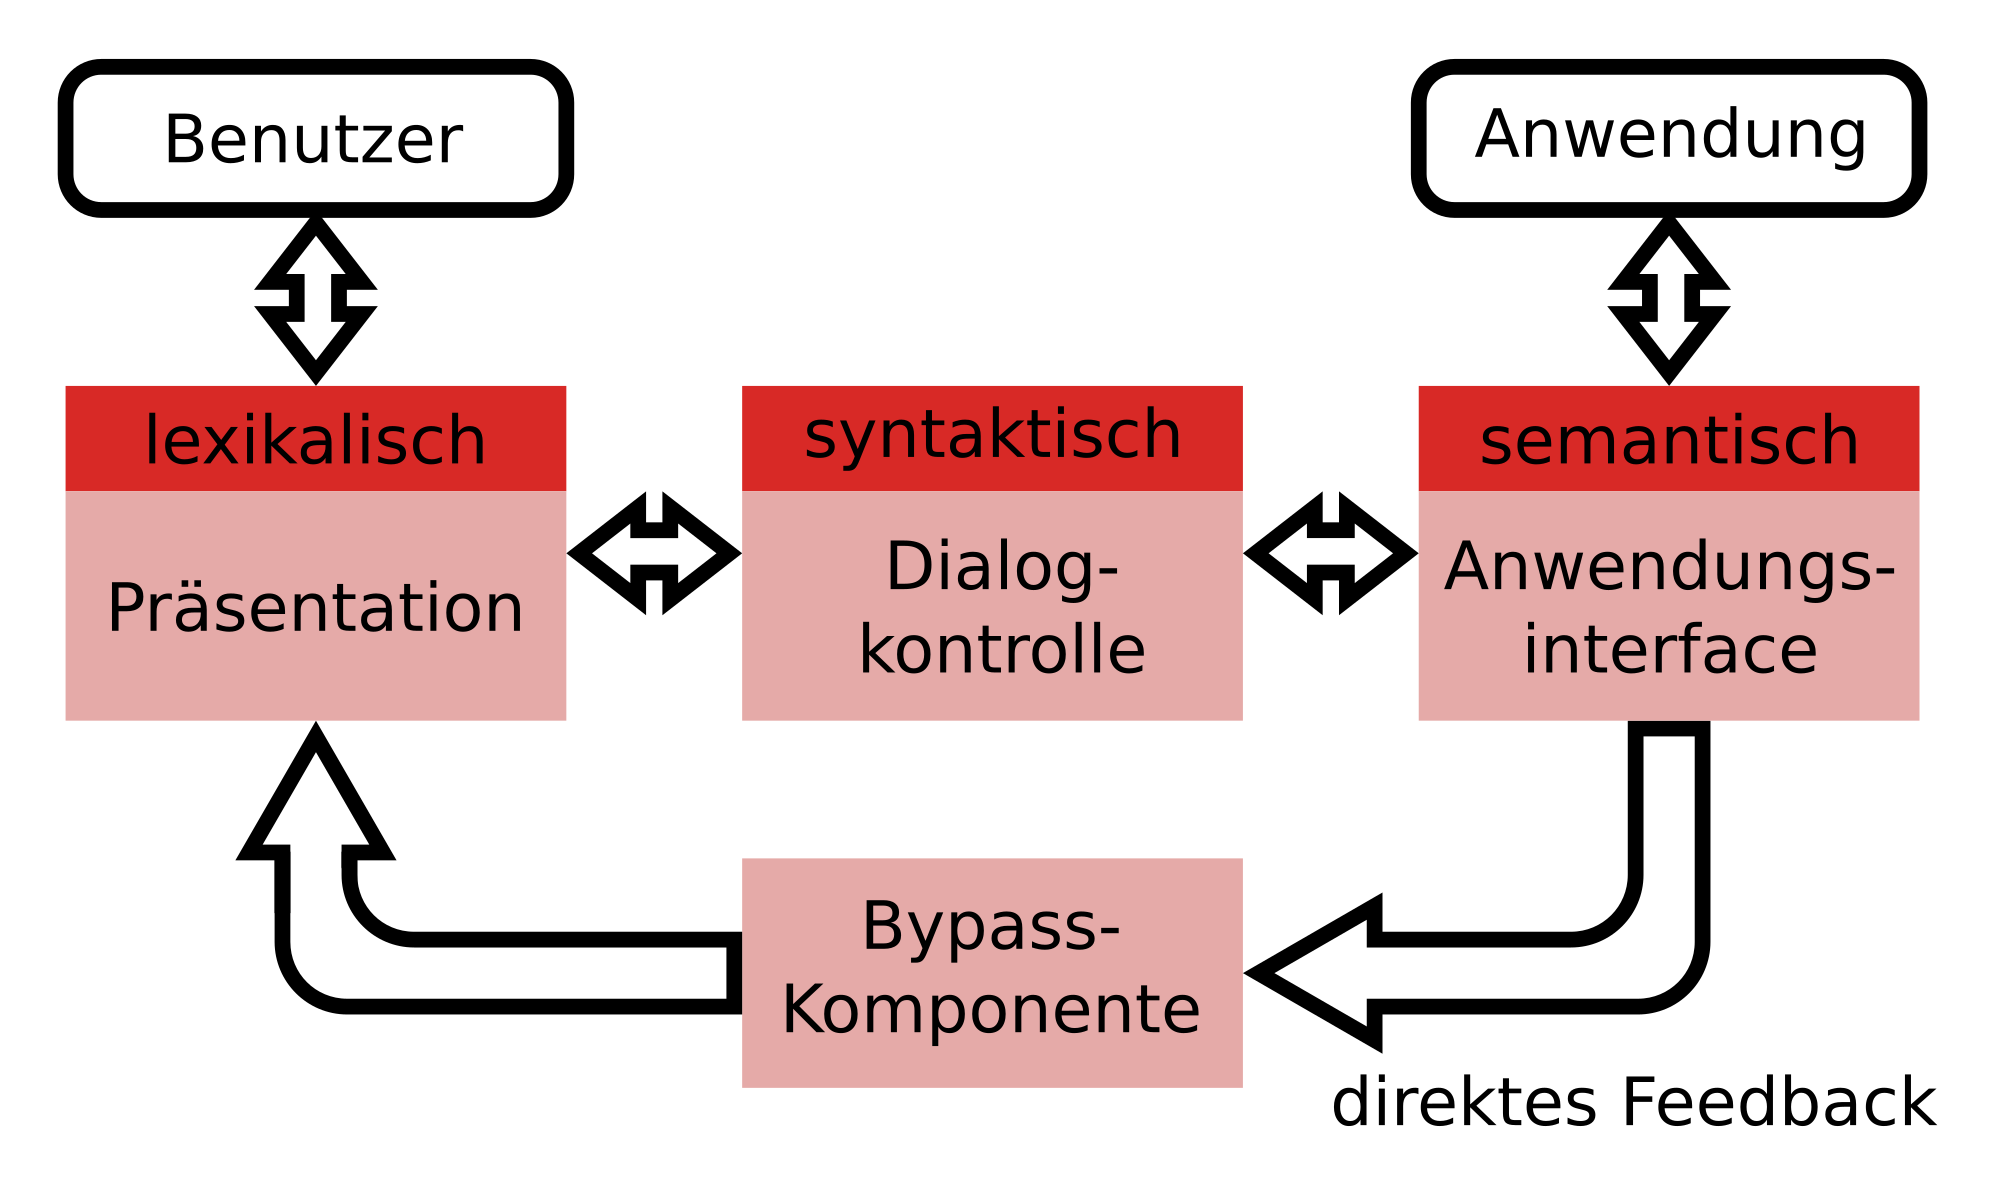
\includegraphics[width=0.7\linewidth]{./Documents/Graphics/SeeheimModel.png}
	\end{center}
	\subsubsection{Presentation-Abstraction-Control}
	\begin{description}
		\item[Presentation] Syntax der Interaktion mit der Anwendung
		      (I/O, wie er vom Nutzer wahrgenommen wird)
		\item[Abstraction] Semantik der Interaktion
		\item[Control]  Konsistenz von Presentation und Abstraction
	\end{description}
	\begin{center}
		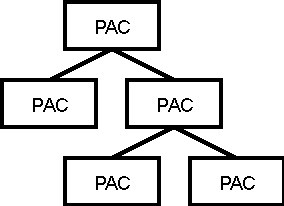
\includegraphics[width=0.5\linewidth]{./Documents/Graphics/DiagramPAC.pdf}
	\end{center}
	\textit{Vorteil:} Wartbarkeit; Austausch von Objekten \\
	\textit{Nachteil:} Dekomponierung der Interaktion fordernd;
	Verarbeitungsaufwand
	\subsubsection{Model-View-Controller (MVC)}
	\begin{description}
		\item[Model] Datenhaltung und Geschäftslogik
		\item[View] Darstellung der Daten
		\item[Controller] Steuerung der Anwendung
	\end{description}
	\begin{center}
		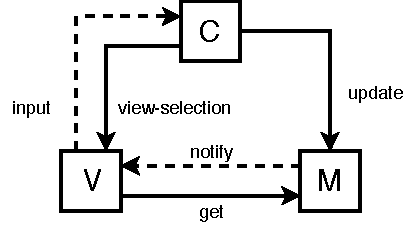
\includegraphics[width=0.7\linewidth]{./Documents/Graphics/DiagramMVC.pdf}
	\end{center}
	Beobachter-Pattern: View beobachtet Model; Controller kann View austauschen,
	Kommandos im Modell ausführen, Model ändern
	\paragraph{Front Controller} \emph{(Fowler)} \par
	Durch die Steigende Komplexität der Web-Anwendungen wird ein
	seitenspezifischer Controller eingeführt. D.h. Ein Zentraler Zugangspunkt
	zuständig für Weiterleitungen, welche mit Hilfe von Tabellenerfolgt. Ein
	Spezifischer Page-Controller generiert im nächsten Schritt die View.
	\subsubsection{Model-View-Presenter}
	\paragraph{Potel}
	\begin{center}
		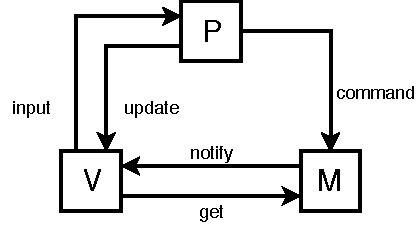
\includegraphics[width=0.7\linewidth]{./Documents/Graphics/DiagramMVPPotel.pdf}
	\end{center}
	\paragraph{Fowler}
	Das Model-View-Presenter Passive View nach Fowler präsentiert die Aufgaben
	der mit MVC eingeführten Komponenten, dabei beachtet der Presenter das Modell
	und der Presenter aktualisiert die View.
	\begin{center}
		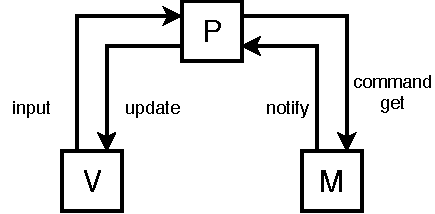
\includegraphics[width=0.7\linewidth]{./Documents/Graphics/DiagramMVPFowler.pdf}
	\end{center}
	\subsubsection{Model-ViewModel-Model (MVVM)}
	Das MVVM Modell ist eine im Wesentlichen aus MVC und MVP abgeleitete
	Spezialisierung anhand technischer Merkmale von WPF.
	(Stärkung der Separation of Concerns durch XAML; Beschreibt die Einbindung
	von Events und Bindings)
	\begin{center}
		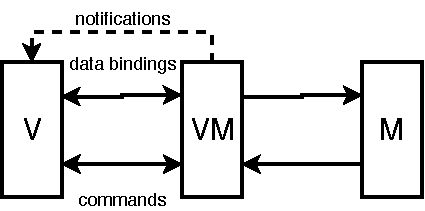
\includegraphics[width=0.7\linewidth]{./Documents/Graphics/DiagramMVVM.pdf}
	\end{center}
	\section{Frameworks und Tools}
	\subsection{Frameworks}
	Programmiergerüst für die Softwareentwicklung\\
	(z.B. .NET Framework)
	\subsection{Klassifizierung anhand\\Entwicklungsansatz}
	{
		\setlength{\columnseprule}{0pt}
		\begin{multicols*}{2}
			\paragraph{Black-Box}
			\begin{itemize}
				\item Ansatz
				      \begin{itemize}[leftmargin=4pt,nolistsep]
					      \item Vordefinirte Komponenten
					      \item Komponenten werden durch ihre Schnittstelle
					            beschrieben
					      \item Verständnis der internen Funktionsweise der
					            Komponenten \emph{nicht} erforderlich
				      \end{itemize}
				\item Anwendung des Frameworks
				      \begin{itemize}[leftmargin=4pt,nolistsep]
					      \item Objektkomposition
				      \end{itemize}
				\item Vorteil
				      \begin{itemize}[leftmargin=4pt,nolistsep]
					      \item Niedrige Einarbeitungszeit
				      \end{itemize}
			\end{itemize}
			\columnbreak
			\paragraph{White-Box}
			\begin{itemize}
				\item Ansatz
				      \begin{itemize}[leftmargin=4pt,nolistsep]
					      \item Vordefinirte Komponenten und/oder Codebausteine
					      \item Verständnis der internen Funktionsweise der Komponenten
					            erforderlich
				      \end{itemize}
				\item Anwendung des Frameworks
				      \begin{itemize}[leftmargin=4pt,nolistsep]
					      \item z.B. Erweiterungen des Frameworks durch Ableitungen
					      \item z.B. Verknüpfen mit Callbacks von Komponenten des Frameworks
				      \end{itemize}
				\item Vorteil
				      \begin{itemize}[leftmargin=4pt,nolistsep]
					      \item Hohe Flexibilität
				      \end{itemize}
			\end{itemize}
		\end{multicols*}
	}
	\subsection{Klassifizierung nach Einsatzbereich}
	\begin{itemize}
		\item Toolkit
		      \begin{itemize}[nolistsep]
			      \item Unterstützt die \textbf{Erstellung} einer
			            Benutzerschnittstelle durch wiederverwendbare
			            Komponenten (z.B. Menüs, Buttons)
			      \item Erscheinungsbild und Verhalten der GUI-Komponenten
			            vorgegeben, u.U. anpassbar
		      \end{itemize}
		\item Interface Builder
		      \begin{itemize}[nolistsep]
			      \item Baut auf einem Toolkit auf
			      \item Unterstützen (i.A. graphischen) \textbf{Entwurf} und
			            \textbf{Erstellung} der Benutzerschnittstelle ohne
			            Programmieraufwand
		      \end{itemize}
		\item User Interface Management System (UIMS)
		      \begin{itemize}[nolistsep]
			      \item Vermitteln zwischen Benutzer und Anwendungsprogrammen
			      \item Unterstützen \textbf{Entwurf}, \textbf{Erstellung} und
			            \textbf{Pflege} von Benutzerschnittstellen
			      \item Umfassen daher Toolkit und Interface Builder
		      \end{itemize}
	\end{itemize}
	\subsection{Prototyping}
	Prototyping: Realisieren ausgewählte Aspekte eines UI mit dem Ziel Feedback
	der Benutzer vor der detaillierten Umsetzung eines Interaktionskonzepts
	einzuholen und so frühes und kontinuierliches Testen zu befördern
	\subsection{Modellbasierte Entwicklung}
	\begin{itemize}
		\item Horizontale Prototypen
		      \begin{itemize}[nolistsep]
			      \item Breite Ausdehnung
			      \item Enthalten vollständige Benutzerschnittstelle aber keine
			            Funktionalität
		      \end{itemize}
		\item Vertikale Prototypen
		      \begin{itemize}[nolistsep]
			      \item Tiefe Ausdehnung
			      \item Enthalten Funktionalität, aber nur einen Teil der
			            Benutzerschnittstelle
		      \end{itemize}
	\end{itemize}
	\subsubsection{Unterscheidung hinsichtlich\\Übereinstimmung}
	{
		\setlength{\columnseprule}{0pt}
		\begin{multicols*}{2}
			\paragraph{Low Fidelity}
			\begin{itemize}
				\item Zweck
				      \begin{itemize}[leftmargin=4pt,nolistsep]
					      \item Testen von Ideen, Abläufen
				      \end{itemize}
				\item Vorteile
				      \begin{itemize}[leftmargin=4pt,nolistsep]
					      \item Einfaches und schnelles Erstellen
					      \item Keine Programmierkenntnisse notwendig
					      \item Änderungen sind schnell herbeizuführen
				      \end{itemize}
			\end{itemize}
			\columnbreak
			\paragraph{High Fidelity}
			\begin{itemize}
				\item Zweck
				      \begin{itemize}[leftmargin=4pt,nolistsep]
					      \item Testen von UI-Umsetztung nahe dem finalen
					            Produkt
				      \end{itemize}
				\item Vorteil
				      \begin{itemize}[leftmargin=4pt,nolistsep]
					      \item Geringe Abstraktion gegenüber dem finalen
					            Produkt
					      \item Testen in realer Arbeitsumgebung möglich
					      \item Zusammenspiel zwischen UI und Anwendung kann
					            getestet werden
				      \end{itemize}
			\end{itemize}
		\end{multicols*}
	}
	\paragraph{Techniken} Storyboards und Interface Flow Diagram (Low Fidelity),
	Mockups (High Fidelity), Wireframes (Low Fidelity)
	\subsection{Modellbasierte Entwicklung}
	Das \textbf{Ziel} ist die Flexibilisierung von der Design-Phase
	(Entwicklungsprozess) und der Runtime-Phase (im Wirkbetrieb)
	\paragraph{Ansatz}
	\begin{itemize}
		\item Aspekte der Benutzerschnittstelle durch Modelle
		      plattformunabhängig beschreiben
		\item Modelle als Eingabe für eine automatische Generierung der
		      Benutzerschnittstelle verwenden
		\item Änderungen der Anforderungen im Modell, nicht im Code
		\item Vermeiden von Inkonsistenzen zwischen Modell und Code als Folge
		      händischer Überführung
	\end{itemize}
	\subsubsection{Modelltypen im\\Cameleon-Reference-Framework}
	\begin{itemize}
		\item Domain-Modell
		      \begin{itemize}[nolistsep]
			      \item Concepts: Konzepte die im Anwendungsgebiet vorkommen
			      \item Tasks: Aufgaben, die der Benutzer durchzuführen hat
		      \end{itemize}
		\item Context-of-Use-Modell
		      \begin{itemize}[nolistsep]
			      \item User: Benutzer und Rollen im zu unterstützenden
			            Arbeitsablauf
			      \item Platform: Technische Möglichkeiten und Grenzen
			            involvierter Geräte; Interaktion von Geräten im
			            Anwendungskontext;
			            Verfügbare Interaktionskomponenten (Presentation Model)
			      \item Environment: Umgebung, in der die Anwendung genutzt wird
		      \end{itemize}
		\item Adaption-Modell
		      \begin{itemize}[nolistsep]
			      \item Evolution: Zu welcher Benutzerschnittstelle soll
			            gewechselt werden und welches Transition Model soll
			            verwendet werden
			      \item Transition: Wie soll der Übergang zwischen zwei
			            Benutzerschnittschnellen dem Benutzer kommuniziert
			            werden
		      \end{itemize}
	\end{itemize}
\end{multicols*}
\begin{multicols*}{3}
	\section{Windows Presentation Foundation}
	\lstinputlisting{Documents/Programs/Example.xaml}
	\lstinputlisting{Documents/Programs/Example.cs}
	\subsection{Events}
	\lstinputlisting{Documents/Programs/Events.xaml}
	\lstinputlisting{Documents/Programs/Events.cs}
	\subsubsection{Routed Events}
	Routed Events pflanzen sich entweder aufwärts oder abwärts in der Hierarchie
	des \emph{Visual Trees} der GUI fort: Zwischen drin liegende Layout-Manager
	(\texttt{Grid}, \texttt{StackPanel}, etc.) bekommen nur dann ein Event, wenn
	ein enthaltendes Elementen ebenfalls ein Event geschickt bekommt. Bei \(\ge\)
	2 sich überlagernden Elementen in der gleichen Ebene wählt das Hit-Testing
	\emph{immer} das im XAML \emph{zuletzt} deklarierte.
	\begin{itemize}
		\item Direkte Events (werden nicht weitergereicht)
		      \begin{itemize}[nolistsep]
			      \item Ereignisse werden nur von dem Element verarbeitet, bei
			            dem sie auch aufgetreten sind (konform mit .NET)
		      \end{itemize}
		\item Bubbling-Events
		      \begin{itemize}[nolistsep]
			      \item Event wird zuerst an den Handler des Quellelements
			            weitergereicht. Dann wird sich dieses Weiterreichen
			            elementweise bis zur Wurzel fortgesetzt (meist Window)
		      \end{itemize}
		\item Tunneling Events
		      \begin{itemize}[nolistsep]
			      \item Hier ist es umgekehrt wie beim Bubbling. Die
			            Ereigniskette beginnt beim Wurzelelement, d.h. Window
			            oder Page. Nachfolgend der Handler des
			            untergeordneten Elements usw.
		      \end{itemize}
		\item Bubbling/Tunneling stoppen: \texttt{args.Handled = true;}
	\end{itemize}
	\subsection{Attribut-Element-Syntax}
	\lstinputlisting{Documents/Programs/Attribute_1.xaml}
	\lstinputlisting{Documents/Programs/Attribute_2.xaml}
	\subsection{Bindings}
	Bindungen binden immer nur auf \textbf{Properties}, nicht auf
	Member-Variablen, und der angegebene \textit{Path} muss \texttt{public} sein.
	\subsubsection{Richtungsbestimmung}
	\begin{itemize}
		\item \textit{TwoWay}: Zweiwegebindung
		\item \textit{OneWay}: Von der Quelle zum Ziel
		\item \textit{OneWayToSource}: Von dem Ziel zur Quelle
		\item \textit{OneTime}: Eine einmalige \textit{OneWay} Bindung
	\end{itemize}
	\subsubsection{Data-Context}
	\lstinputlisting{Documents/Programs/DataContext.cs}
	\lstinputlisting{Documents/Programs/DataContext.xaml}
	\columnbreak
	\subsubsection{INotifyPropertyChanged}
	\lstinputlisting{Documents/Programs/NotifyProperty.cs}
	\subsection{Style Templates}
	\lstinputlisting{Documents/Programs/Styles.xaml}
	\subsection{Triggers und Validation}
	\lstinputlisting{Documents/Programs/Triggers.xaml}
	\lstinputlisting{Documents/Programs/Validation.xaml}
\end{multicols*}
\end{document}
